% section
\section{Implementation} \label{section::implementation}
 This section describes the structure and usage of the implemented baselines (Shi et al. \cite{Shi2015}, Patraucean et al. \cite{Patraucean2015},
 Lotter et al. \cite{Lotter2016}), so that the reader is able to understand the given code and is able to redo the experiments and even extend the code to
 his own needs.
  
 % subsection
 \subsection{Structure} \label{subsection::structure}
  The code is structured in a way, that everyone without specific knowledge of coding should be able to get the necessary files and results as easy as possible and
  everyone with more experience in coding should have a nice structure to add or remove certain methods.
  \\\\
  The first important files are the setup.py and requirements.txt. Both of them are useful to install every necessary requirement to run the code on someones 
  local machine or on any machine learning cloud computing platform. This was tested by during the experiments on a private computer, on 
  \href{www.floydhub.com} {Floydhub} and \href{colab.research.google.com}{Google Colab}.
  For Google Colab one needs to add a Jupyter notebook file \cite{Kluyver2016}, which is not included in the thesis.
  \\\\
  The part where all comes together is the main file in the PredNet folder, in which the main method is started. This main method controls the whole
  execution, such as initializing the network,
  initializing the optimizer (Adam \cite{Kingma2015} or RMSProp \cite{Ruder2016}) and starting the training or testing. Testing, training and validation methods 
  are seperated in own files, so the user has more 
  control over the methods itself (For example, the user wants to validate on more then one error, but wants to test on only one, he can simply
  add the change to the validation file, without interchanging with any other method.). Everything related to the actual network models is stored in the model 
  folder, which stores the three baselines and the folder for all submodules of which they consist (For example, PredNet has the error module, which is stored in 
  model/modules/error.py.). Many useful methods, e.g. the choose of a certain error function can be found in the helper folder. The dataset files are stored in 
  data, as well as some simple scripts to fetch and pre-process the data. There is also the dataset folder, which holds the \href{https://pytorch.org/docs/stable/
  data.html}{PyTorch dataloader} files. The code is able to save and load models, so one is able to continue training at a certain point, or test the network
  after training, those network files are stored in the mdl folder. To overcome the problem of having the need to change network parameters always inside the
  code files, I implemented a solution, which offers the user to simply add \href{https://yaml.org/}{yml}-files which contain every necessary information about 
  the network parameters, where to store the model and the logs, using debug mode and where the dataset files are stored. Those files are stored in the yml 
  folder. To log the training, validation and test results, I am using Tensorboard \cite{tensorflow2015}. Those files are stored in the log folder.
  Lastly one is able to create the backpropagation graph from the used network. This is outputted into the graph folder.
  A tree graph of the structure is given in the appendix~\ref{section::appendix}.
  
 % subsection
 \subsection{Usage}
  The usage is also structured in a way, that everyone should be able to change mostly every parameter without having the need of changing lines of code.
  The code is started using the console with plenty of different mandatory and optional parameters.
  \begin{figure}[H]
   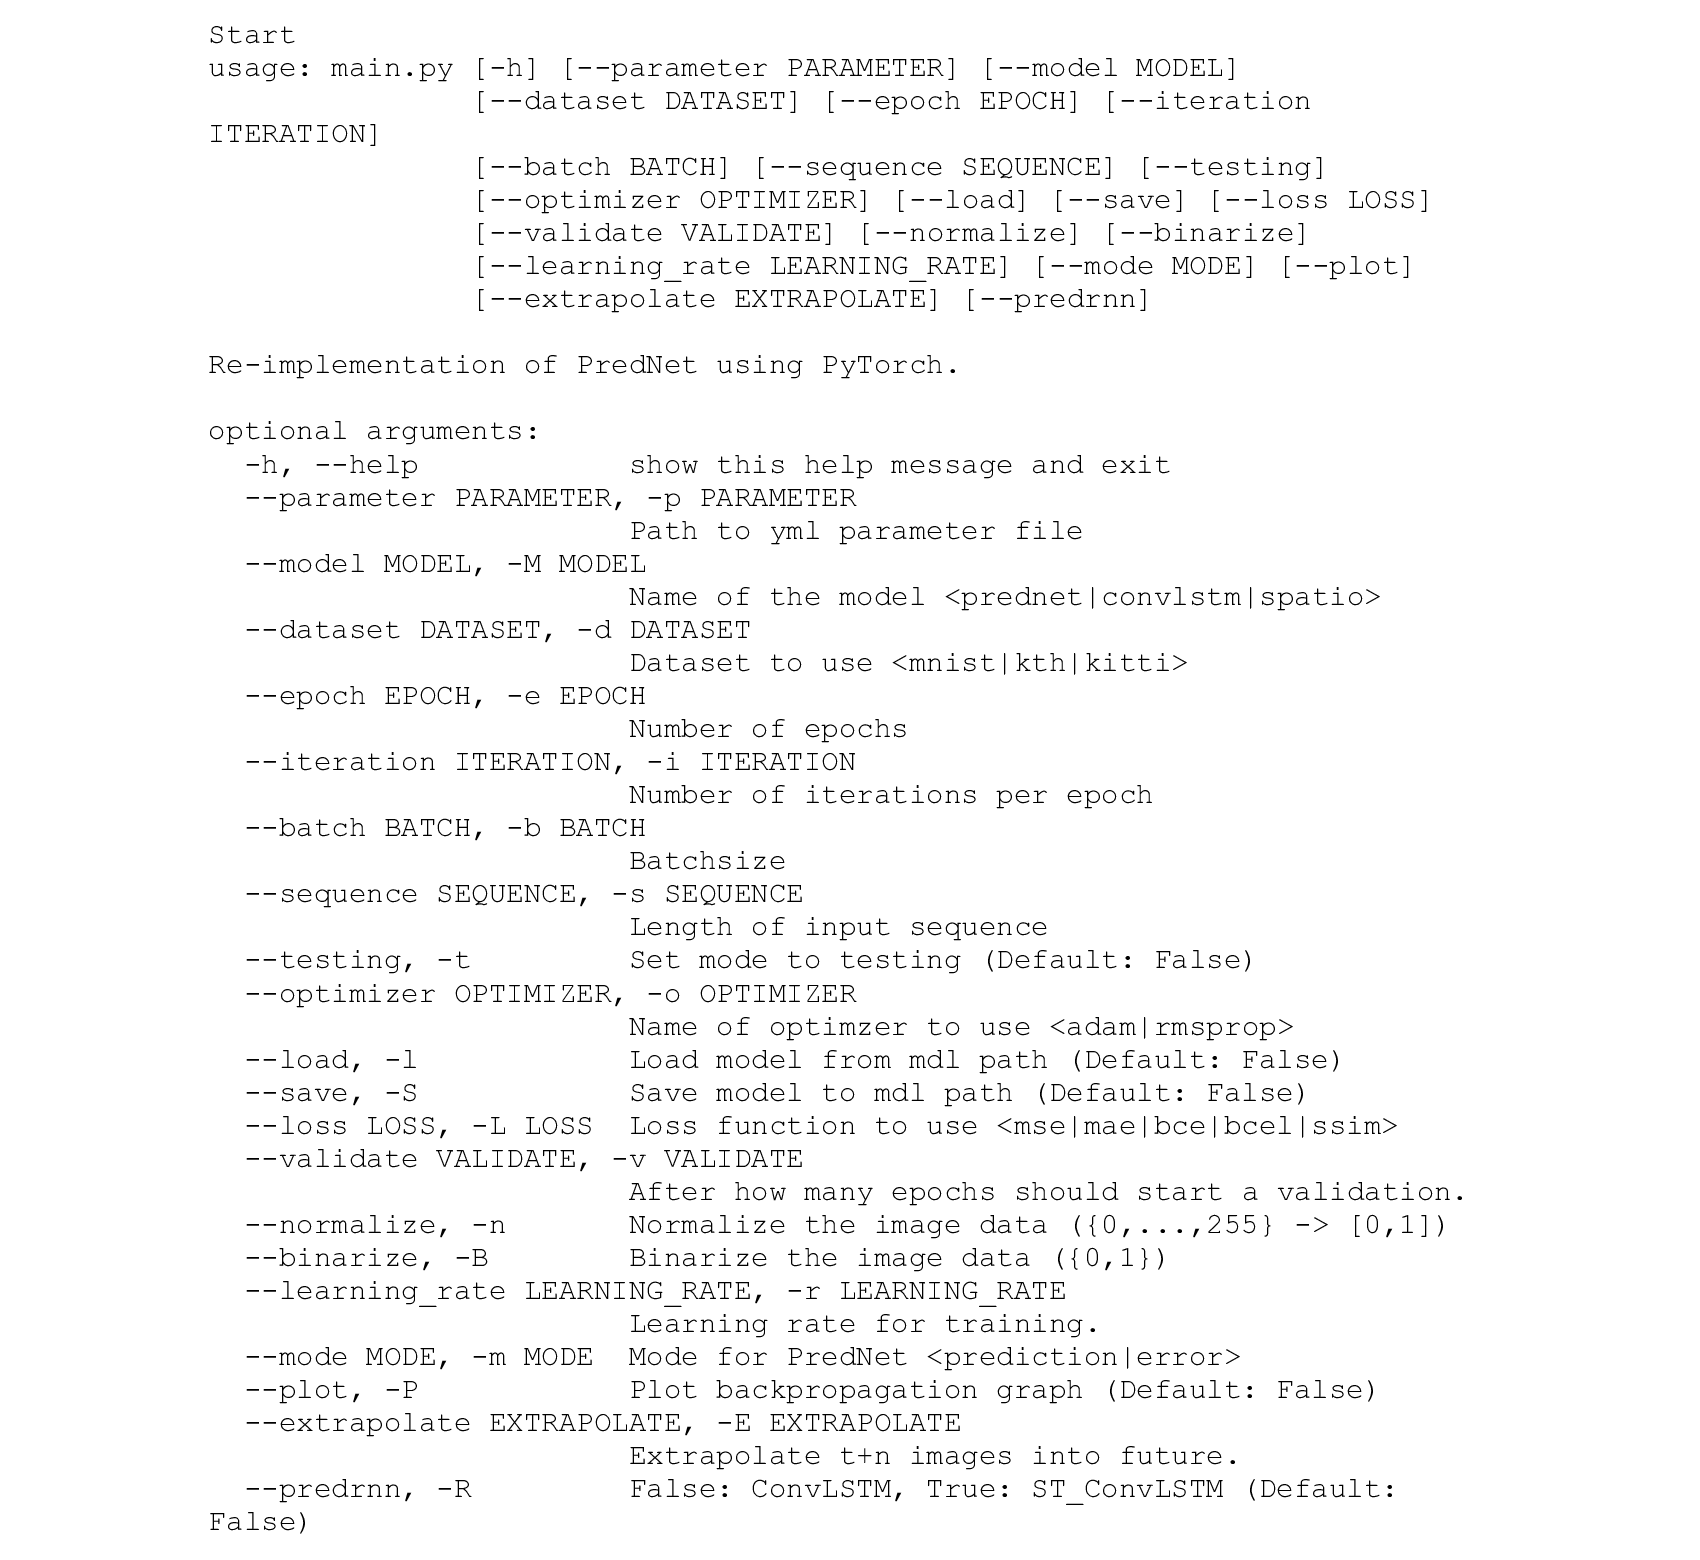
\includegraphics[width=1.0\textwidth]{../Images/usage.png}
   \centering
   \caption{Usage of Implementation}
   \label{fig:tree}
  \end{figure}\noindent
